\section{Math}

\subsection{math subsection 1}
\lipsum[1]

\subsection{math subsection 2}
% First figure: Paraboloid
\begin{figure}[htbp]
\centering
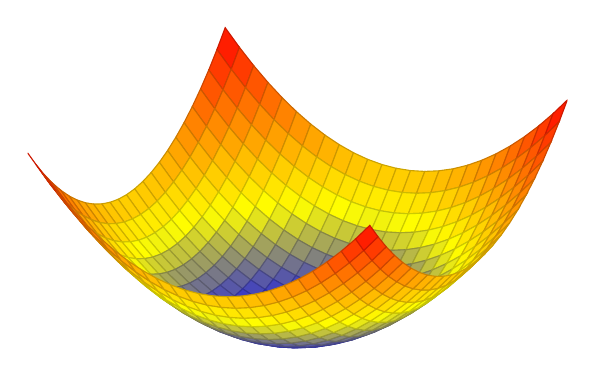
\begin{tikzpicture}
  \begin{axis}[
    title={},
    hide axis,
    view={120}{30}
  ]
  \addplot3[
    surf,
    domain=-2:2,
    domain y=-2:2,
  ]
  {x^2 + y^2};
  \end{axis}
\end{tikzpicture}
\caption{A Paraboloid Surface}
\label{fig:paraboloid}
\end{figure}

As shown in Figure \ref{fig:paraboloid}, the points make up a surface called a paraboloid. It is the shape of the parabola \( z = x^2 \) rotated about the \( z \) axis.

% Second figure: Hemisphere
\begin{figure}[h]
\centering
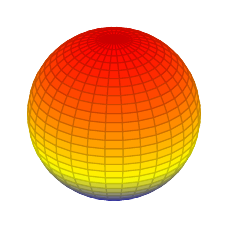
\begin{tikzpicture}
  \begin{axis}[
    title={},
    hide axis,
    view={120}{30},
    axis equal
  ]
  \addplot3[
    domain=0:180,
    domain y=0:360,
    samples=31,
    samples y=31,
    surf,
    z buffer=sort
  ] (
    {sin(x)*cos(y)},
    {sin(x)*sin(y)},
    {cos(x)}
  );
  \end{axis}
\end{tikzpicture}
\caption{A Hemispherical Surface}
\label{fig:hemisphere}
\end{figure}

Figure \ref{fig:hemisphere} illustrates a hemisphere, showcasing how a spherical surface can be represented in a three-dimensional space.

$$ \sum_{n = 1}^{\infty}$$